% Created by tikzDevice version 0.12.3.2 on 2022-02-18 15:43:45
% !TEX encoding = UTF-8 Unicode
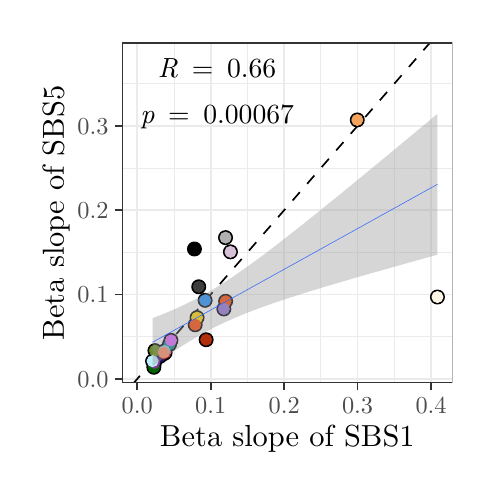
\begin{tikzpicture}[x=1pt,y=1pt]
\definecolor{fillColor}{RGB}{255,255,255}
\path[use as bounding box,fill=fillColor,fill opacity=0.00] (0,0) rectangle (158.99,158.99);
\begin{scope}
\path[clip] (  0.00,  0.00) rectangle (158.99,158.99);
\definecolor{drawColor}{RGB}{255,255,255}
\definecolor{fillColor}{RGB}{255,255,255}

\path[draw=drawColor,line width= 0.6pt,line join=round,line cap=round,fill=fillColor] (  0.00,  0.00) rectangle (158.99,158.99);
\end{scope}
\begin{scope}
\path[clip] ( 34.16, 30.69) rectangle (153.49,153.49);
\definecolor{fillColor}{RGB}{255,255,255}

\path[fill=fillColor] ( 34.16, 30.69) rectangle (153.49,153.49);
\definecolor{drawColor}{gray}{0.92}

\path[draw=drawColor,line width= 0.3pt,line join=round] ( 34.16, 47.30) --
	(153.49, 47.30);

\path[draw=drawColor,line width= 0.3pt,line join=round] ( 34.16, 77.79) --
	(153.49, 77.79);

\path[draw=drawColor,line width= 0.3pt,line join=round] ( 34.16,108.28) --
	(153.49,108.28);

\path[draw=drawColor,line width= 0.3pt,line join=round] ( 34.16,138.77) --
	(153.49,138.77);

\path[draw=drawColor,line width= 0.3pt,line join=round] ( 52.85, 30.69) --
	( 52.85,153.49);

\path[draw=drawColor,line width= 0.3pt,line join=round] ( 79.40, 30.69) --
	( 79.40,153.49);

\path[draw=drawColor,line width= 0.3pt,line join=round] (105.95, 30.69) --
	(105.95,153.49);

\path[draw=drawColor,line width= 0.3pt,line join=round] (132.50, 30.69) --
	(132.50,153.49);

\path[draw=drawColor,line width= 0.6pt,line join=round] ( 34.16, 32.05) --
	(153.49, 32.05);

\path[draw=drawColor,line width= 0.6pt,line join=round] ( 34.16, 62.54) --
	(153.49, 62.54);

\path[draw=drawColor,line width= 0.6pt,line join=round] ( 34.16, 93.03) --
	(153.49, 93.03);

\path[draw=drawColor,line width= 0.6pt,line join=round] ( 34.16,123.52) --
	(153.49,123.52);

\path[draw=drawColor,line width= 0.6pt,line join=round] ( 39.58, 30.69) --
	( 39.58,153.49);

\path[draw=drawColor,line width= 0.6pt,line join=round] ( 66.13, 30.69) --
	( 66.13,153.49);

\path[draw=drawColor,line width= 0.6pt,line join=round] ( 92.68, 30.69) --
	( 92.68,153.49);

\path[draw=drawColor,line width= 0.6pt,line join=round] (119.22, 30.69) --
	(119.22,153.49);

\path[draw=drawColor,line width= 0.6pt,line join=round] (145.77, 30.69) --
	(145.77,153.49);
\definecolor{drawColor}{RGB}{0,0,0}

\path[draw=drawColor,line width= 0.6pt,dash pattern=on 4pt off 4pt ,line join=round] ( 11.67,  0.00) -- (150.11,158.99);
\definecolor{fillColor}{RGB}{0,0,0}

\path[draw=drawColor,line width= 0.4pt,line join=round,line cap=round,fill=fillColor] ( 61.21, 54.21) circle (  2.50);

\path[draw=drawColor,line width= 0.4pt,line join=round,line cap=round,fill=fillColor] ( 49.66, 41.53) circle (  2.50);

\path[draw=drawColor,line width= 0.4pt,line join=round,line cap=round,fill=fillColor] ( 61.81, 65.36) circle (  2.50);

\path[draw=drawColor,line width= 0.4pt,line join=round,line cap=round,fill=fillColor] ( 73.27, 77.98) circle (  2.50);

\path[draw=drawColor,line width= 0.4pt,line join=round,line cap=round,fill=fillColor] ( 71.49, 83.12) circle (  2.50);

\path[draw=drawColor,line width= 0.4pt,line join=round,line cap=round,fill=fillColor] ( 47.77, 40.18) circle (  2.50);

\path[draw=drawColor,line width= 0.4pt,line join=round,line cap=round,fill=fillColor] ( 64.12, 60.47) circle (  2.50);

\path[draw=drawColor,line width= 0.4pt,line join=round,line cap=round,fill=fillColor] ( 49.25, 41.21) circle (  2.50);

\path[draw=drawColor,line width= 0.4pt,line join=round,line cap=round,fill=fillColor] ( 64.49, 46.23) circle (  2.50);

\path[draw=drawColor,line width= 0.4pt,line join=round,line cap=round,fill=fillColor] ( 71.53, 60.13) circle (  2.50);

\path[draw=drawColor,line width= 0.4pt,line join=round,line cap=round,fill=fillColor] ( 60.53, 51.63) circle (  2.50);

\path[draw=drawColor,line width= 0.4pt,line join=round,line cap=round,fill=fillColor] ( 45.59, 36.27) circle (  2.50);

\path[draw=drawColor,line width= 0.4pt,line join=round,line cap=round,fill=fillColor] (148.07, 61.66) circle (  2.50);

\path[draw=drawColor,line width= 0.4pt,line join=round,line cap=round,fill=fillColor] ( 45.99, 42.30) circle (  2.50);

\path[draw=drawColor,line width= 0.4pt,line join=round,line cap=round,fill=fillColor] (119.10,125.64) circle (  2.50);

\path[draw=drawColor,line width= 0.4pt,line join=round,line cap=round,fill=fillColor] ( 51.25, 44.56) circle (  2.50);

\path[draw=drawColor,line width= 0.4pt,line join=round,line cap=round,fill=fillColor] ( 45.81, 37.86) circle (  2.50);

\path[draw=drawColor,line width= 0.4pt,line join=round,line cap=round,fill=fillColor] ( 51.78, 46.00) circle (  2.50);

\path[draw=drawColor,line width= 0.4pt,line join=round,line cap=round,fill=fillColor] ( 49.41, 42.15) circle (  2.50);

\path[draw=drawColor,line width= 0.4pt,line join=round,line cap=round,fill=fillColor] ( 60.26, 79.02) circle (  2.50);

\path[draw=drawColor,line width= 0.4pt,line join=round,line cap=round,fill=fillColor] ( 45.13, 38.48) circle (  2.50);

\path[draw=drawColor,line width= 0.4pt,line join=round,line cap=round,fill=fillColor] ( 70.89, 57.35) circle (  2.50);

\path[draw=drawColor,line width= 0.4pt,line join=round,line cap=round,fill=fillColor] ( 49.21, 41.60) circle (  2.50);
\definecolor{drawColor}{RGB}{255,215,0}
\definecolor{fillColor}{RGB}{255,215,0}

\path[draw=drawColor,line width= 0.4pt,line join=round,line cap=round,fill=fillColor] ( 61.21, 54.21) circle (  1.96);
\definecolor{drawColor}{RGB}{205,96,144}
\definecolor{fillColor}{RGB}{205,96,144}

\path[draw=drawColor,line width= 0.4pt,line join=round,line cap=round,fill=fillColor] ( 49.66, 41.53) circle (  1.96);
\definecolor{drawColor}{gray}{0.24}
\definecolor{fillColor}{gray}{0.24}

\path[draw=drawColor,line width= 0.4pt,line join=round,line cap=round,fill=fillColor] ( 61.81, 65.36) circle (  1.96);
\definecolor{drawColor}{RGB}{216,191,216}
\definecolor{fillColor}{RGB}{216,191,216}

\path[draw=drawColor,line width= 0.4pt,line join=round,line cap=round,fill=fillColor] ( 73.27, 77.98) circle (  1.96);
\definecolor{drawColor}{gray}{0.69}
\definecolor{fillColor}{gray}{0.69}

\path[draw=drawColor,line width= 0.4pt,line join=round,line cap=round,fill=fillColor] ( 71.49, 83.12) circle (  1.96);
\definecolor{drawColor}{RGB}{25,25,112}
\definecolor{fillColor}{RGB}{25,25,112}

\path[draw=drawColor,line width= 0.4pt,line join=round,line cap=round,fill=fillColor] ( 47.77, 40.18) circle (  1.96);
\definecolor{drawColor}{RGB}{30,144,255}
\definecolor{fillColor}{RGB}{30,144,255}

\path[draw=drawColor,line width= 0.4pt,line join=round,line cap=round,fill=fillColor] ( 64.12, 60.47) circle (  1.96);
\definecolor{drawColor}{RGB}{139,35,35}
\definecolor{fillColor}{RGB}{139,35,35}

\path[draw=drawColor,line width= 0.4pt,line join=round,line cap=round,fill=fillColor] ( 49.25, 41.21) circle (  1.96);
\definecolor{drawColor}{RGB}{179,47,11}
\definecolor{fillColor}{RGB}{179,47,11}

\path[draw=drawColor,line width= 0.4pt,line join=round,line cap=round,fill=fillColor] ( 64.49, 46.23) circle (  1.96);
\definecolor{drawColor}{RGB}{255,69,0}
\definecolor{fillColor}{RGB}{255,69,0}

\path[draw=drawColor,line width= 0.4pt,line join=round,line cap=round,fill=fillColor] ( 71.53, 60.13) circle (  1.96);

\path[draw=drawColor,line width= 0.4pt,line join=round,line cap=round,fill=fillColor] ( 60.53, 51.63) circle (  1.96);
\definecolor{drawColor}{RGB}{0,100,0}
\definecolor{fillColor}{RGB}{0,100,0}

\path[draw=drawColor,line width= 0.4pt,line join=round,line cap=round,fill=fillColor] ( 45.59, 36.27) circle (  1.96);
\definecolor{drawColor}{RGB}{253,245,230}
\definecolor{fillColor}{RGB}{253,245,230}

\path[draw=drawColor,line width= 0.4pt,line join=round,line cap=round,fill=fillColor] (148.07, 61.66) circle (  1.96);
\definecolor{drawColor}{RGB}{105,139,34}
\definecolor{fillColor}{RGB}{105,139,34}

\path[draw=drawColor,line width= 0.4pt,line join=round,line cap=round,fill=fillColor] ( 45.99, 42.30) circle (  1.96);
\definecolor{drawColor}{RGB}{244,163,93}
\definecolor{fillColor}{RGB}{244,163,93}

\path[draw=drawColor,line width= 0.4pt,line join=round,line cap=round,fill=fillColor] (119.10,125.64) circle (  1.96);
\definecolor{drawColor}{RGB}{0,139,139}
\definecolor{fillColor}{RGB}{0,139,139}

\path[draw=drawColor,line width= 0.4pt,line join=round,line cap=round,fill=fillColor] ( 51.25, 44.56) circle (  1.96);
\definecolor{drawColor}{RGB}{122,55,139}
\definecolor{fillColor}{RGB}{122,55,139}

\path[draw=drawColor,line width= 0.4pt,line join=round,line cap=round,fill=fillColor] ( 45.81, 37.86) circle (  1.96);
\definecolor{drawColor}{RGB}{224,102,255}
\definecolor{fillColor}{RGB}{224,102,255}

\path[draw=drawColor,line width= 0.4pt,line join=round,line cap=round,fill=fillColor] ( 51.78, 46.00) circle (  1.96);
\definecolor{drawColor}{RGB}{135,206,250}
\definecolor{fillColor}{RGB}{135,206,250}

\path[draw=drawColor,line width= 0.4pt,line join=round,line cap=round,fill=fillColor] ( 49.41, 42.15) circle (  1.96);
\definecolor{drawColor}{RGB}{0,0,0}
\definecolor{fillColor}{RGB}{0,0,0}

\path[draw=drawColor,line width= 0.4pt,line join=round,line cap=round,fill=fillColor] ( 60.26, 79.02) circle (  1.96);
\definecolor{drawColor}{RGB}{191,239,255}
\definecolor{fillColor}{RGB}{191,239,255}

\path[draw=drawColor,line width= 0.4pt,line join=round,line cap=round,fill=fillColor] ( 45.13, 38.48) circle (  1.96);
\definecolor{drawColor}{RGB}{147,112,219}
\definecolor{fillColor}{RGB}{147,112,219}

\path[draw=drawColor,line width= 0.4pt,line join=round,line cap=round,fill=fillColor] ( 70.89, 57.35) circle (  1.96);
\definecolor{drawColor}{RGB}{255,140,105}
\definecolor{fillColor}{RGB}{255,140,105}

\path[draw=drawColor,line width= 0.4pt,line join=round,line cap=round,fill=fillColor] ( 49.21, 41.60) circle (  1.96);
\definecolor{fillColor}{RGB}{153,153,153}

\path[fill=fillColor,fill opacity=0.40] ( 45.13, 54.01) --
	( 46.43, 54.51) --
	( 47.73, 55.02) --
	( 49.04, 55.54) --
	( 50.34, 56.08) --
	( 51.64, 56.63) --
	( 52.95, 57.19) --
	( 54.25, 57.77) --
	( 55.55, 58.37) --
	( 56.86, 58.98) --
	( 58.16, 59.62) --
	( 59.46, 60.27) --
	( 60.76, 60.94) --
	( 62.07, 61.63) --
	( 63.37, 62.35) --
	( 64.67, 63.08) --
	( 65.98, 63.83) --
	( 67.28, 64.60) --
	( 68.58, 65.40) --
	( 69.89, 66.21) --
	( 71.19, 67.04) --
	( 72.49, 67.89) --
	( 73.80, 68.75) --
	( 75.10, 69.63) --
	( 76.40, 70.53) --
	( 77.70, 71.44) --
	( 79.01, 72.36) --
	( 80.31, 73.30) --
	( 81.61, 74.24) --
	( 82.92, 75.20) --
	( 84.22, 76.16) --
	( 85.52, 77.14) --
	( 86.83, 78.12) --
	( 88.13, 79.11) --
	( 89.43, 80.11) --
	( 90.74, 81.11) --
	( 92.04, 82.12) --
	( 93.34, 83.13) --
	( 94.64, 84.15) --
	( 95.95, 85.18) --
	( 97.25, 86.21) --
	( 98.55, 87.24) --
	( 99.86, 88.27) --
	(101.16, 89.31) --
	(102.46, 90.36) --
	(103.77, 91.40) --
	(105.07, 92.45) --
	(106.37, 93.50) --
	(107.67, 94.55) --
	(108.98, 95.61) --
	(110.28, 96.67) --
	(111.58, 97.72) --
	(112.89, 98.79) --
	(114.19, 99.85) --
	(115.49,100.91) --
	(116.80,101.98) --
	(118.10,103.05) --
	(119.40,104.11) --
	(120.71,105.18) --
	(122.01,106.25) --
	(123.31,107.33) --
	(124.61,108.40) --
	(125.92,109.47) --
	(127.22,110.55) --
	(128.52,111.62) --
	(129.83,112.70) --
	(131.13,113.78) --
	(132.43,114.86) --
	(133.74,115.94) --
	(135.04,117.01) --
	(136.34,118.10) --
	(137.65,119.18) --
	(138.95,120.26) --
	(140.25,121.34) --
	(141.55,122.42) --
	(142.86,123.51) --
	(144.16,124.59) --
	(145.46,125.67) --
	(146.77,126.76) --
	(148.07,127.84) --
	(148.07, 76.95) --
	(146.77, 76.59) --
	(145.46, 76.23) --
	(144.16, 75.87) --
	(142.86, 75.51) --
	(141.55, 75.15) --
	(140.25, 74.78) --
	(138.95, 74.42) --
	(137.65, 74.06) --
	(136.34, 73.69) --
	(135.04, 73.33) --
	(133.74, 72.96) --
	(132.43, 72.60) --
	(131.13, 72.23) --
	(129.83, 71.86) --
	(128.52, 71.49) --
	(127.22, 71.12) --
	(125.92, 70.75) --
	(124.61, 70.38) --
	(123.31, 70.01) --
	(122.01, 69.64) --
	(120.71, 69.26) --
	(119.40, 68.89) --
	(118.10, 68.51) --
	(116.80, 68.13) --
	(115.49, 67.75) --
	(114.19, 67.37) --
	(112.89, 66.99) --
	(111.58, 66.60) --
	(110.28, 66.22) --
	(108.98, 65.83) --
	(107.67, 65.44) --
	(106.37, 65.05) --
	(105.07, 64.65) --
	(103.77, 64.26) --
	(102.46, 63.86) --
	(101.16, 63.45) --
	( 99.86, 63.05) --
	( 98.55, 62.64) --
	( 97.25, 62.23) --
	( 95.95, 61.81) --
	( 94.64, 61.39) --
	( 93.34, 60.96) --
	( 92.04, 60.53) --
	( 90.74, 60.10) --
	( 89.43, 59.65) --
	( 88.13, 59.21) --
	( 86.83, 58.75) --
	( 85.52, 58.29) --
	( 84.22, 57.82) --
	( 82.92, 57.34) --
	( 81.61, 56.85) --
	( 80.31, 56.35) --
	( 79.01, 55.84) --
	( 77.70, 55.32) --
	( 76.40, 54.78) --
	( 75.10, 54.23) --
	( 73.80, 53.67) --
	( 72.49, 53.09) --
	( 71.19, 52.49) --
	( 69.89, 51.87) --
	( 68.58, 51.24) --
	( 67.28, 50.59) --
	( 65.98, 49.92) --
	( 64.67, 49.23) --
	( 63.37, 48.51) --
	( 62.07, 47.78) --
	( 60.76, 47.03) --
	( 59.46, 46.25) --
	( 58.16, 45.46) --
	( 56.86, 44.65) --
	( 55.55, 43.82) --
	( 54.25, 42.97) --
	( 52.95, 42.10) --
	( 51.64, 41.22) --
	( 50.34, 40.33) --
	( 49.04, 39.42) --
	( 47.73, 38.50) --
	( 46.43, 37.56) --
	( 45.13, 36.62) --
	cycle;

\path[] ( 45.13, 54.01) --
	( 46.43, 54.51) --
	( 47.73, 55.02) --
	( 49.04, 55.54) --
	( 50.34, 56.08) --
	( 51.64, 56.63) --
	( 52.95, 57.19) --
	( 54.25, 57.77) --
	( 55.55, 58.37) --
	( 56.86, 58.98) --
	( 58.16, 59.62) --
	( 59.46, 60.27) --
	( 60.76, 60.94) --
	( 62.07, 61.63) --
	( 63.37, 62.35) --
	( 64.67, 63.08) --
	( 65.98, 63.83) --
	( 67.28, 64.60) --
	( 68.58, 65.40) --
	( 69.89, 66.21) --
	( 71.19, 67.04) --
	( 72.49, 67.89) --
	( 73.80, 68.75) --
	( 75.10, 69.63) --
	( 76.40, 70.53) --
	( 77.70, 71.44) --
	( 79.01, 72.36) --
	( 80.31, 73.30) --
	( 81.61, 74.24) --
	( 82.92, 75.20) --
	( 84.22, 76.16) --
	( 85.52, 77.14) --
	( 86.83, 78.12) --
	( 88.13, 79.11) --
	( 89.43, 80.11) --
	( 90.74, 81.11) --
	( 92.04, 82.12) --
	( 93.34, 83.13) --
	( 94.64, 84.15) --
	( 95.95, 85.18) --
	( 97.25, 86.21) --
	( 98.55, 87.24) --
	( 99.86, 88.27) --
	(101.16, 89.31) --
	(102.46, 90.36) --
	(103.77, 91.40) --
	(105.07, 92.45) --
	(106.37, 93.50) --
	(107.67, 94.55) --
	(108.98, 95.61) --
	(110.28, 96.67) --
	(111.58, 97.72) --
	(112.89, 98.79) --
	(114.19, 99.85) --
	(115.49,100.91) --
	(116.80,101.98) --
	(118.10,103.05) --
	(119.40,104.11) --
	(120.71,105.18) --
	(122.01,106.25) --
	(123.31,107.33) --
	(124.61,108.40) --
	(125.92,109.47) --
	(127.22,110.55) --
	(128.52,111.62) --
	(129.83,112.70) --
	(131.13,113.78) --
	(132.43,114.86) --
	(133.74,115.94) --
	(135.04,117.01) --
	(136.34,118.10) --
	(137.65,119.18) --
	(138.95,120.26) --
	(140.25,121.34) --
	(141.55,122.42) --
	(142.86,123.51) --
	(144.16,124.59) --
	(145.46,125.67) --
	(146.77,126.76) --
	(148.07,127.84);

\path[] (148.07, 76.95) --
	(146.77, 76.59) --
	(145.46, 76.23) --
	(144.16, 75.87) --
	(142.86, 75.51) --
	(141.55, 75.15) --
	(140.25, 74.78) --
	(138.95, 74.42) --
	(137.65, 74.06) --
	(136.34, 73.69) --
	(135.04, 73.33) --
	(133.74, 72.96) --
	(132.43, 72.60) --
	(131.13, 72.23) --
	(129.83, 71.86) --
	(128.52, 71.49) --
	(127.22, 71.12) --
	(125.92, 70.75) --
	(124.61, 70.38) --
	(123.31, 70.01) --
	(122.01, 69.64) --
	(120.71, 69.26) --
	(119.40, 68.89) --
	(118.10, 68.51) --
	(116.80, 68.13) --
	(115.49, 67.75) --
	(114.19, 67.37) --
	(112.89, 66.99) --
	(111.58, 66.60) --
	(110.28, 66.22) --
	(108.98, 65.83) --
	(107.67, 65.44) --
	(106.37, 65.05) --
	(105.07, 64.65) --
	(103.77, 64.26) --
	(102.46, 63.86) --
	(101.16, 63.45) --
	( 99.86, 63.05) --
	( 98.55, 62.64) --
	( 97.25, 62.23) --
	( 95.95, 61.81) --
	( 94.64, 61.39) --
	( 93.34, 60.96) --
	( 92.04, 60.53) --
	( 90.74, 60.10) --
	( 89.43, 59.65) --
	( 88.13, 59.21) --
	( 86.83, 58.75) --
	( 85.52, 58.29) --
	( 84.22, 57.82) --
	( 82.92, 57.34) --
	( 81.61, 56.85) --
	( 80.31, 56.35) --
	( 79.01, 55.84) --
	( 77.70, 55.32) --
	( 76.40, 54.78) --
	( 75.10, 54.23) --
	( 73.80, 53.67) --
	( 72.49, 53.09) --
	( 71.19, 52.49) --
	( 69.89, 51.87) --
	( 68.58, 51.24) --
	( 67.28, 50.59) --
	( 65.98, 49.92) --
	( 64.67, 49.23) --
	( 63.37, 48.51) --
	( 62.07, 47.78) --
	( 60.76, 47.03) --
	( 59.46, 46.25) --
	( 58.16, 45.46) --
	( 56.86, 44.65) --
	( 55.55, 43.82) --
	( 54.25, 42.97) --
	( 52.95, 42.10) --
	( 51.64, 41.22) --
	( 50.34, 40.33) --
	( 49.04, 39.42) --
	( 47.73, 38.50) --
	( 46.43, 37.56) --
	( 45.13, 36.62);
\definecolor{drawColor}{RGB}{51,102,255}

\path[draw=drawColor,line width= 0.2pt,line join=round] ( 45.13, 45.31) --
	( 46.43, 46.04) --
	( 47.73, 46.76) --
	( 49.04, 47.48) --
	( 50.34, 48.20) --
	( 51.64, 48.93) --
	( 52.95, 49.65) --
	( 54.25, 50.37) --
	( 55.55, 51.09) --
	( 56.86, 51.82) --
	( 58.16, 52.54) --
	( 59.46, 53.26) --
	( 60.76, 53.98) --
	( 62.07, 54.71) --
	( 63.37, 55.43) --
	( 64.67, 56.15) --
	( 65.98, 56.87) --
	( 67.28, 57.60) --
	( 68.58, 58.32) --
	( 69.89, 59.04) --
	( 71.19, 59.77) --
	( 72.49, 60.49) --
	( 73.80, 61.21) --
	( 75.10, 61.93) --
	( 76.40, 62.66) --
	( 77.70, 63.38) --
	( 79.01, 64.10) --
	( 80.31, 64.82) --
	( 81.61, 65.55) --
	( 82.92, 66.27) --
	( 84.22, 66.99) --
	( 85.52, 67.71) --
	( 86.83, 68.44) --
	( 88.13, 69.16) --
	( 89.43, 69.88) --
	( 90.74, 70.60) --
	( 92.04, 71.33) --
	( 93.34, 72.05) --
	( 94.64, 72.77) --
	( 95.95, 73.49) --
	( 97.25, 74.22) --
	( 98.55, 74.94) --
	( 99.86, 75.66) --
	(101.16, 76.38) --
	(102.46, 77.11) --
	(103.77, 77.83) --
	(105.07, 78.55) --
	(106.37, 79.27) --
	(107.67, 80.00) --
	(108.98, 80.72) --
	(110.28, 81.44) --
	(111.58, 82.16) --
	(112.89, 82.89) --
	(114.19, 83.61) --
	(115.49, 84.33) --
	(116.80, 85.05) --
	(118.10, 85.78) --
	(119.40, 86.50) --
	(120.71, 87.22) --
	(122.01, 87.95) --
	(123.31, 88.67) --
	(124.61, 89.39) --
	(125.92, 90.11) --
	(127.22, 90.84) --
	(128.52, 91.56) --
	(129.83, 92.28) --
	(131.13, 93.00) --
	(132.43, 93.73) --
	(133.74, 94.45) --
	(135.04, 95.17) --
	(136.34, 95.89) --
	(137.65, 96.62) --
	(138.95, 97.34) --
	(140.25, 98.06) --
	(141.55, 98.78) --
	(142.86, 99.51) --
	(144.16,100.23) --
	(145.46,100.95) --
	(146.77,101.67) --
	(148.07,102.40);
\definecolor{drawColor}{RGB}{0,0,0}

\node[text=drawColor,anchor=base west,inner sep=0pt, outer sep=0pt, scale=  1.00] at ( 47.07,141.05) {\itshape R};

\node[text=drawColor,anchor=base west,inner sep=0pt, outer sep=0pt, scale=  1.00] at ( 54.33,141.05) { };

\node[text=drawColor,anchor=base west,inner sep=0pt, outer sep=0pt, scale=  1.00] at ( 59.31,141.05) {=};

\node[text=drawColor,anchor=base west,inner sep=0pt, outer sep=0pt, scale=  1.00] at ( 67.05,141.05) { };

\node[text=drawColor,anchor=base west,inner sep=0pt, outer sep=0pt, scale=  1.00] at ( 72.03,141.05) {0.66};

\node[text=drawColor,anchor=base west,inner sep=0pt, outer sep=0pt, scale=  1.00] at ( 40.69,124.23) {\itshape p};

\node[text=drawColor,anchor=base west,inner sep=0pt, outer sep=0pt, scale=  1.00] at ( 45.78,124.23) { };

\node[text=drawColor,anchor=base west,inner sep=0pt, outer sep=0pt, scale=  1.00] at ( 50.76,124.23) {=};

\node[text=drawColor,anchor=base west,inner sep=0pt, outer sep=0pt, scale=  1.00] at ( 58.50,124.23) { };

\node[text=drawColor,anchor=base west,inner sep=0pt, outer sep=0pt, scale=  1.00] at ( 63.48,124.23) {0.00067};
\definecolor{drawColor}{gray}{0.20}

\path[draw=drawColor,line width= 0.6pt,line join=round,line cap=round] ( 34.16, 30.69) rectangle (153.49,153.49);
\end{scope}
\begin{scope}
\path[clip] (  0.00,  0.00) rectangle (158.99,158.99);
\definecolor{drawColor}{gray}{0.30}

\node[text=drawColor,anchor=base east,inner sep=0pt, outer sep=0pt, scale=  0.88] at ( 29.21, 29.02) {0.0};

\node[text=drawColor,anchor=base east,inner sep=0pt, outer sep=0pt, scale=  0.88] at ( 29.21, 59.51) {0.1};

\node[text=drawColor,anchor=base east,inner sep=0pt, outer sep=0pt, scale=  0.88] at ( 29.21, 90.00) {0.2};

\node[text=drawColor,anchor=base east,inner sep=0pt, outer sep=0pt, scale=  0.88] at ( 29.21,120.49) {0.3};
\end{scope}
\begin{scope}
\path[clip] (  0.00,  0.00) rectangle (158.99,158.99);
\definecolor{drawColor}{gray}{0.20}

\path[draw=drawColor,line width= 0.6pt,line join=round] ( 31.41, 32.05) --
	( 34.16, 32.05);

\path[draw=drawColor,line width= 0.6pt,line join=round] ( 31.41, 62.54) --
	( 34.16, 62.54);

\path[draw=drawColor,line width= 0.6pt,line join=round] ( 31.41, 93.03) --
	( 34.16, 93.03);

\path[draw=drawColor,line width= 0.6pt,line join=round] ( 31.41,123.52) --
	( 34.16,123.52);
\end{scope}
\begin{scope}
\path[clip] (  0.00,  0.00) rectangle (158.99,158.99);
\definecolor{drawColor}{gray}{0.20}

\path[draw=drawColor,line width= 0.6pt,line join=round] ( 39.58, 27.94) --
	( 39.58, 30.69);

\path[draw=drawColor,line width= 0.6pt,line join=round] ( 66.13, 27.94) --
	( 66.13, 30.69);

\path[draw=drawColor,line width= 0.6pt,line join=round] ( 92.68, 27.94) --
	( 92.68, 30.69);

\path[draw=drawColor,line width= 0.6pt,line join=round] (119.22, 27.94) --
	(119.22, 30.69);

\path[draw=drawColor,line width= 0.6pt,line join=round] (145.77, 27.94) --
	(145.77, 30.69);
\end{scope}
\begin{scope}
\path[clip] (  0.00,  0.00) rectangle (158.99,158.99);
\definecolor{drawColor}{gray}{0.30}

\node[text=drawColor,anchor=base,inner sep=0pt, outer sep=0pt, scale=  0.88] at ( 39.58, 19.68) {0.0};

\node[text=drawColor,anchor=base,inner sep=0pt, outer sep=0pt, scale=  0.88] at ( 66.13, 19.68) {0.1};

\node[text=drawColor,anchor=base,inner sep=0pt, outer sep=0pt, scale=  0.88] at ( 92.68, 19.68) {0.2};

\node[text=drawColor,anchor=base,inner sep=0pt, outer sep=0pt, scale=  0.88] at (119.22, 19.68) {0.3};

\node[text=drawColor,anchor=base,inner sep=0pt, outer sep=0pt, scale=  0.88] at (145.77, 19.68) {0.4};
\end{scope}
\begin{scope}
\path[clip] (  0.00,  0.00) rectangle (158.99,158.99);
\definecolor{drawColor}{RGB}{0,0,0}

\node[text=drawColor,anchor=base,inner sep=0pt, outer sep=0pt, scale=  1.10] at ( 93.83,  7.64) {Beta slope of SBS1};
\end{scope}
\begin{scope}
\path[clip] (  0.00,  0.00) rectangle (158.99,158.99);
\definecolor{drawColor}{RGB}{0,0,0}

\node[text=drawColor,rotate= 90.00,anchor=base,inner sep=0pt, outer sep=0pt, scale=  1.10] at ( 13.08, 92.09) {Beta slope of SBS5};
\end{scope}
\end{tikzpicture}
